\section{Lecture 11: Multi-Core and GPU}
\subsection{Multi-Core Computers}
Integration of several cores on a single chip, this is a cheap and simple solution to gain more parellel computing. This has also been called \textbf{Chip Multiprocessor}. A \textbf{MIMD processor} have different cores operating on different sets of data. In a \textbf{shared memory multiprocessor}, all cores share the same memory via some cache system.

Pros:
\begin{itemize}
\item High power consumption in relation to performance gained (2-3\% power increase when 1\% performance increase).
\item Power generates heat and cooling is expensive.
\item Instruction Level Parallelism only
\item General trend in computer architecture -> shift towards more parallelism.
\newline
\end{itemize}

Cons:
\begin{itemize}
\item Design time and complexity increased due to complex methods to increase ILP.
\item Many new applications are multithreaded, e.g. Multimedia applications.
\item Much faster cache coherency circuits, in a single chip.
\item Smaller in physical size than SMP.
\end{itemize}

The idea of multicores processor can be seen in figure \ref{fig:simple-multi-model}.

\begin{figure}[H]
  \centering
  \scalebox{0.6}{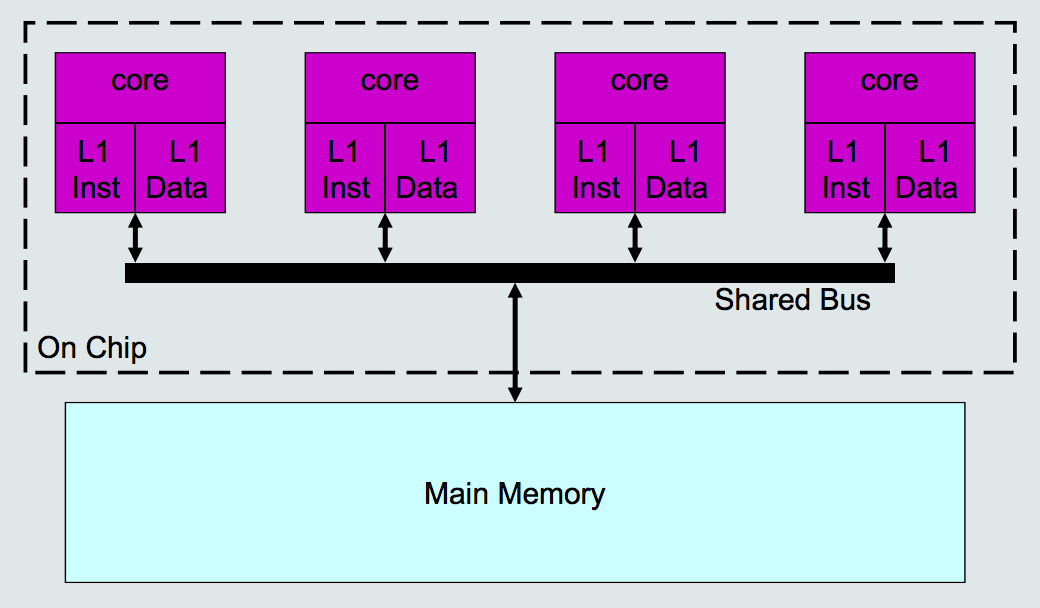
\includegraphics{img/simple-multi-model.png}}
  \caption{A simplified model of a multicore processor.}
  \label{fig:simple-multi-model}
\end{figure}

There are also lots of other ideas of how this can be implemented, some of these can be seen in figure \ref{fig:multi-core-ideas}

\begin{figure}[H]
  \centering
  \scalebox{0.4}{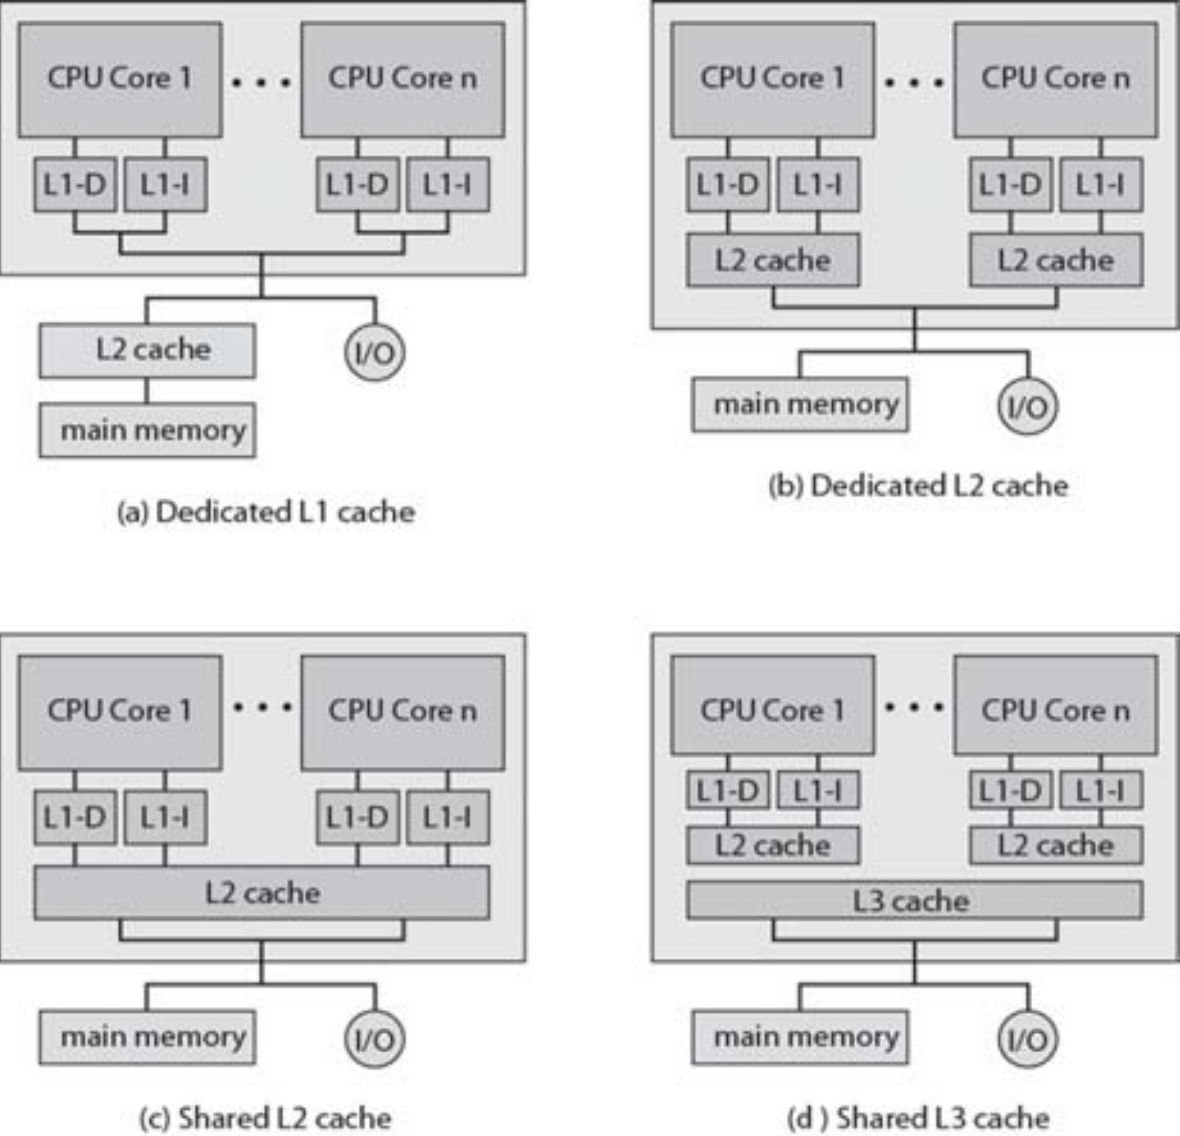
\includegraphics{img/multi-core-ideas.png}}
  \caption{Some different ideas of how to implement multicore processors.}
  \label{fig:multi-core-ideas}
\end{figure}


\subsubsection{Intel Core i7}
This is a processor with the concept of both several cores and several threads (multithreads).

A simple schedule of the architecture can be seen in figure \ref{fig:intel-i7} 

\begin{figure}[H]
  \centering
  \scalebox{0.4}{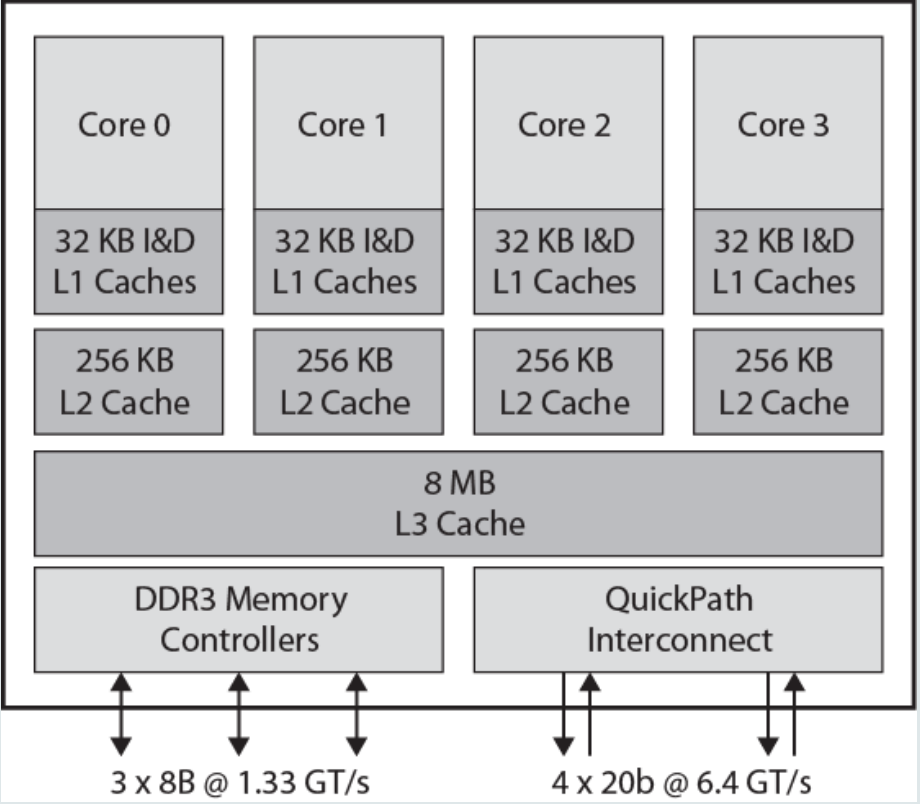
\includegraphics{img/intel-i7.png}}
  \caption{Intel i7 architecture.}
  \label{fig:intel-i7}
\end{figure}
\newpage

\begin{itemize}
\item Four or six identical x86 processors. 
\item Each with their own L1 \& L2 cache.
\item Shared L3 cache.
\item \textbf{Front side bus} (FSB) have been replaced by \textbf{QuickPath Interconnect} QPI to increase the bandwidth between cores.
\item Up to 4 GHz clock frequency.
\end{itemize}

\subsubsection{Intel Polaris}
This processor is developed in cooperation bewtween Linköping University and Intel. It has 80 cores running on one chip, it runs at tFLOPS ($10^{12}$) performance, making it the first ever chip to perform at that level.

\begin{itemize}
\item Its peak power efficiency is 19.4 gFLOPS/Watt (almost 10X better than supercomputers).
\item Workload-aware power management
  \begin{itemize}
  \item The individual computing engines and data routers in each core can be activated or put to sleep based on the performance required by the applications.
  \end{itemize}
\item Mesh network-on-a-chip.
  \begin{itemize}
  \item The cores are connected in a 2D mesh network that implement message-passing. 
  \end{itemize}
\item Frequency target at 5 GHz.
\item Peak of 1.01 Teraflops at 62 watts.
\item Short design time (regularity).
  \begin{itemize}
  \item The tiled-design approach allows designers to use smaller cores that can easily be repeated across the chip. 
  \end{itemize}
\end{itemize}


\subsection{Multithreading}

\subsubsection{Thread-Level Parallelism (TLP)}
Parallelism on a larger level than instruction level parallelism ILP. Instruction stream is divided into smaller streams (threads) that will be executed in parallel. Each thread has its own instructions and data. It is also more cost-effective than ILP.

This technique is very suitable for multi-core arhcitectures, as they can use multiple instruction streams to improve the throughput of computers that run several programs.

\subsubsection{Multithreading Approaches}
\todo{jag förstår inte riktigt det här? finns massvis med förklarande bilder som dessvärre inte förklarar så bra i slides} \\
%https://en.wikipedia.org/wiki/Multithreading_(computer_architecture)
\begin{itemize}

\item Interleaved (fine-grained)
  \begin{itemize}
  \item Processor deals with several thread contexts at a time.
  \item Switching thread at each clock cycle (hardware support needed).
  \item If a thread is blocked, it is skipped.
  \item Hide latency of both short and long pipeline stalls.
  \end{itemize}
  
\item Blocked (coarse-grained)
  \begin{itemize}
  \item Thread executed until an event causes delay (e.g., cache miss).
  \item Relieves the need to have very fast thread switching.
  \item No slow down for ready-to-go threads.
  \end{itemize}
  
\item Simultaneous (SMT)
  \begin{itemize}
  \item Used in \textbf{superscalar architectures}. 
  \item Instructions simultaneously issued from multiple threads to execution units of a superscalar processor.
  \end{itemize}

\item Chip multiprocessing
  \begin{itemize}
  \item Each processor handles separate threads
  \end{itemize}
\end{itemize}

\subsubsection{Interleaved (fine-grained)}
The purpose is to remove all data dependency stalls from the execution pipeline. Since one thread is relatively independent from other threads, there's less chance of one instruction in one pipelining stage needing an output from an older instruction in the pipeline.
\subsubsection{Blocked (coarsed-grained)}
The simplest type of multithreading occurs when one thread runs until it is blocked by an event that normally would create a long-latency stall. Such a stall might be a cache miss that has to access off-chip memory, which might take hundreds of CPU cycles for the data to return. Instead of waiting for the stall to resolve, a threaded processor would switch execution to another thread that was ready to run. Only when the data for the previous thread had arrived, would the previous thread be placed back on the list of ready-to-run threads.

\subsubsection{Simultaneous (SMT)}
The most advanced type of multithreading applies to superscalar processors. Whereas a normal superscalar processor issues multiple instructions from a single thread every CPU cycle, in simultaneous multithreading (SMT) a superscalar processor can issue instructions from multiple threads every CPU cycle. Recognizing that any single thread has a limited amount of instruction-level parallelism, this type of multithreading tries to exploit parallelism available across multiple threads to decrease the waste associated with unused issue slots.

\subsubsection{Scalar Processor Approaches}
\subsubsection{Superscalar Approaches}
\subsubsection{SMT and Chip Multiprocessing}
\subsubsection{Multithreading Paradigms}




\subsection{Graphic Processing Unit (GPU)}
Normal CPUs are designed to handle huge data volumes in serial, one operation at a time (control flow stream).

GPUs instead are designed to handle huge data volumes in parallel in a data stream based flow

When we want to compute a frame for HDTV, there are $2.1*10^(6)$ Pixels that needs to be computed. All of the pixels are independent of each other and we have a lot of spatial locality (regular memory access). This means that we could achieve lots of speedups if we increase the hardware.

Each pixel can take a long time to process, as long as we make sure that we process many of them at the same time. What we need for this is a lot of simple parallel processors running at low clock speed. This means that we focus on a high throughput instead of a low latency.

CPU:
\begin{itemize}
\item Optimized for low latency.
\item A few massive cores, running at very high speeds.
\item Lots of hardware for control, few ALUs.
\end{itemize}

GPU:
\begin{itemize}
\item Optimized for high throughput.
\item A lot of small simple cores, running at low speeds.
\item Lots of ALUs for computation, little hardware for control..
\end{itemize}

The best is to combine these two.
\subsection{General Purpose GPUs}
Very efficient for:
\begin{itemize}
\item Fast parallel floating point processing.
\item SIMD (Single Instruction Multiple Data) operations.
\item High computation per memory access.
\end{itemize}

Not as efficient for
\begin{itemize}
\item Double precision computations.
\item Logical operations on integer data.
\item Random access, memory-intensive operations.
\item Branching-intensive operations
\end{itemize}

GPU control unit fecthes \textbf{1} instruction per clock cycles, and shares it with \textbf{8} processors.

\subsubsection{Divergent Execution}
This is what happens when all the processors mentioned above doesn't want the same instruction. This would really hurt the performance.

An example of this is given in figure \ref{fig:divergent-execution}

\begin{figure}[H]
  \centering
  \scalebox{0.5}{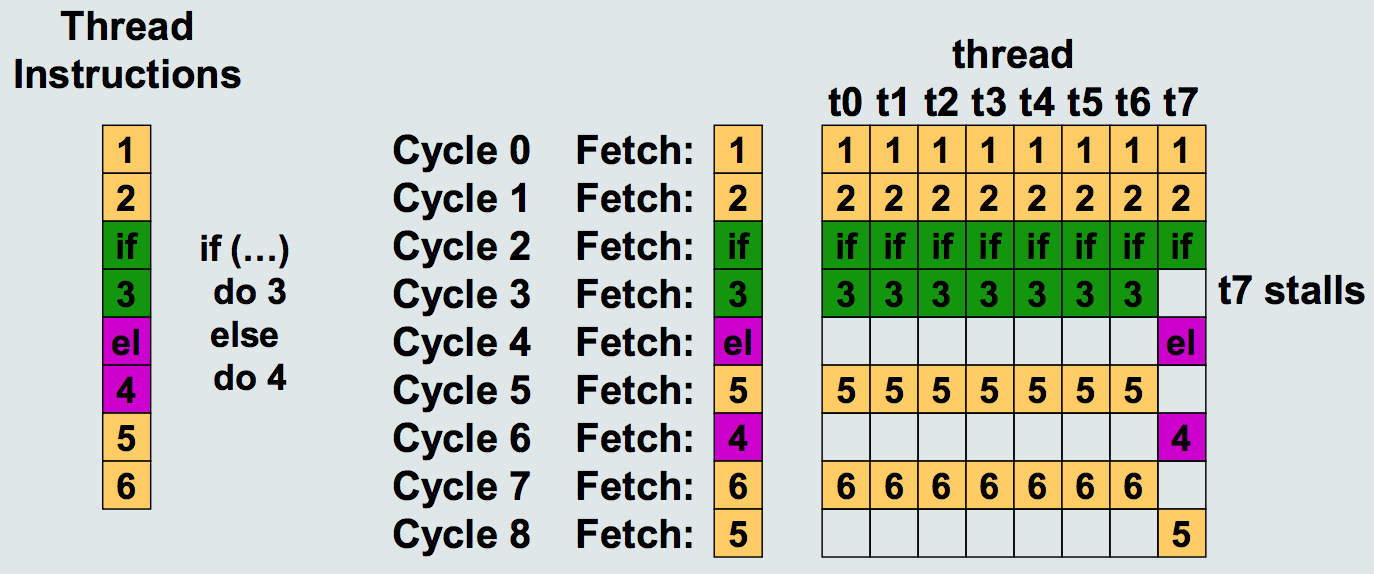
\includegraphics{img/divergent-execution.png}}
  \caption{Divergent execution due to a branch.}
  \label{fig:divergent-execution}
\end{figure}

\subsubsection{Reduce Branch Divergence}
We can reduce these with some software optimizations, such as:
\begin{itemize}
  \item target a divergent branch enclosed by a loop.
  \item execute loop iterations that take the same branch direction.
  \item delay those that take the other direction until later iterations.
  \item execute the delayed operations in future iterations where more threads take the same direction.
\end{itemize}

\subsubsection{GPUPU}
\textbf{General-purpose computing on graphics processing units} is the use of a GPU for doing computations usually handled by the CPU. We can't use any GPU though, it needs to have been provided hardware support to be able to do this. One such GPU is the Intel Tesla.

\subsubsection{NVIDIA Tesla}
Its massively parallel with 1000s of processors,  aswell as cost and power efficient.


\subsubsection{CUDA Programming Language}
\textbf{Computer Unified Device Architecture} is a parallel computing platform and application programming interface (API) model created by NVIDIA. It allows software developers to use a CUDA-enabled graphics processing unit (GPU) for general purpose processing.

It uses an heterogeneous programming approach, serial computation will be handled as usual by the cpu, but parallel computations that are normally handled by the CPU can now be sent to the GPU. An example can be found in the computer game industry, where GPUs are used not only for graphics rendering but also in game physics calculations (physical effects such as debris, smoke, fire, fluids); examples include PhysX and Bullet.

CUDA can not only be used in GPU computing but also in multi-core CPUs, and works especially well with C, C++ and Fortran.

General CUDA steps:
\begin{enumerate}
  \item Copy data from CPU to GPU.
  \item Perform SIMD computations on GPU.
  \item Copy back data from GPU to CPU.
\end{enumerate}

We want to minimize data transfer between CPU \& GPU and maximize the number of threads on the GPU, the execution on host doesn't wait for kernel to finish on GPU.
